%!TEX TS-program = xelatex
\documentclass[]{friggeri-cv}
\usepackage{afterpage}
\usepackage{hyperref}
\usepackage{color}
\usepackage{xcolor}
\usepackage{smartdiagram}
\usepackage{fontspec}
\usepackage{graphicx}
\usepackage{subcaption}


% if you want to add fontawesome package
% you need to compile the tex file with LuaLaTeX
% References:
%   http://texdoc.net/texmf-dist/doc/latex/fontawesome/fontawesome.pdf
%   https://www.ctan.org/tex-archive/fonts/fontawesome?lang=en
%\usepackage{fontawesome}
\usepackage{metalogo}
\usepackage{dtklogos}
\usepackage[utf8]{inputenc}
\usepackage{tikz}
\usetikzlibrary{mindmap,shadows}
\hypersetup{
    pdftitle={},
    pdfauthor={},
    pdfsubject={},
    pdfkeywords={},
    colorlinks=false,           % no lik border color
    allbordercolors=white       % white border color for all
}
\smartdiagramset{
    bubble center node font = \footnotesize,
    bubble node font = \footnotesize,
    % specifies the minimum size of the bubble center node
    bubble center node size = 0.5cm,
    %  specifies the minimum size of the bubbles
    bubble node size = 0.4cm,
    % specifies which is the distance among the bubble center node and the other bubbles
    distance center/other bubbles = 0.29cm,
    % sets the distance from the text to the border of the bubble center node
    distance text center bubble = 0.28cm,
    % set center bubble color
    bubble center node color = pblue,
    % define the list of colors usable in the diagram
    set color list = {lightgray, materialcyan, orange, green, materialorange, materialteal, materialamber, materialindigo, materialgreen, materiallime},
    % sets the opacity at which the bubbles are shown
    bubble fill opacity = 0.6,
    % sets the opacity at which the bubble text is shown
    bubble text opacity = 0.5,
}

\addbibresource{bibliography.bib}
\RequirePackage{xcolor}
\definecolor{pblue}{HTML}{0395DE}

\begin{document}
\header{SiThu}{Thwin}
      {Senior Manager - SRE and Solution Architect}

% Fake text to add separator
\fcolorbox{white}{gray}{\parbox{\dimexpr\textwidth-2\fboxsep-2\fboxrule}{%
.....
}}
%...

% Add badges
\begin{figure}[h]
  \centering
  \begin{subfigure}[b]{0.1\linewidth}
    
\includegraphics[width=\linewidth]{img/cka.png}
  \end{subfigure}
  \begin{subfigure}[b]{0.1\linewidth}
    
\includegraphics[width=\linewidth]{img/istio-expert.png}
  \end{subfigure}
  \begin{subfigure}[b]{0.1\linewidth}
    
\includegraphics[width=\linewidth]{img/istio-intermediate.png}
  \end{subfigure}
  \begin{subfigure}[b]{0.1\linewidth}
    
\includegraphics[width=\linewidth]{img/istio-fundamentals.png}
  \end{subfigure}
  \begin{subfigure}[b]{0.1\linewidth}
    
\includegraphics[width=\linewidth]{img/envoy.png}
  \end{subfigure}
  \begin{subfigure}[b]{0.1\linewidth}
    
\includegraphics[width=\linewidth]{img/ccna.png}
  \end{subfigure}
\end{figure}
%...

% In the aside, each new line forces a line break
\begin{aside}
  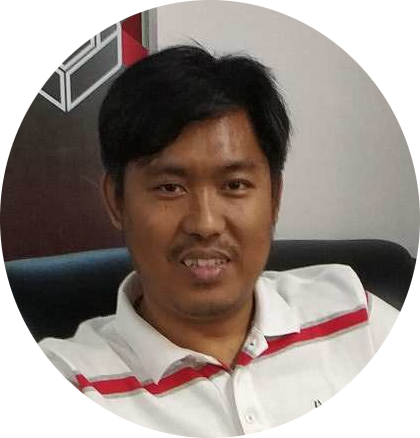
\includegraphics[scale=1]{img/myself-circle.png}
  \section{Traits}
    Quick Learner
    Innovative
  \section{Address}
    CL1-202, Cityloft@Starcity
    Than Lyin Township
    Yangon, Myanmar
    ~
  \section{Contact}
    \textbf{Tel:} +95 979 7969695
    \textbf{Skype:} live:sithuthwin
    ~
  \section{Mail}
    \href{mailto:sithu@thwin.net}{\textbf{sithu@}thwin.net}
    ~
  \section{Social}
    \textbf{LinkedIn:} \href{https://www.linkedin.com/in/si-thu-thwin/}{si-thu-thwin}
    ~
  \section{Web \& Git}
    \href{https://www.thwin.net}{thwin.net}
    \href{https://github.com/herzcthu}{github.com/herzcthu}
    \href{https://gitlab.com/herzcthu}{gitlab.com/herzcthu}
    ~
  % use  \hspace{} or \vspace{} to change bubble size, if needed
  \section{DevSecOps}
    \textbf{GitLab CI/CD}
    \textbf{Terraform/Ansible}
    \textbf{SonarQube}
    \textbf{Maven}
    \textbf{Docker}
    \textbf{ELK/EFK}
    \textbf{Prometheus/Grafana}
    \textbf{K8S/Openshift/Helm/Istio/Single Mesh}
    \textbf{Pinpoint/Zipkin}
    \textbf{PHP}
    \textbf{Python/Flask}
    \textbf{YAML}
    \textbf{Bash}
    \textbf{LaTeX}
    \textbf{gRPC/mTLS/PKI}
    \textbf{AWS/Azure/Oracle}
    \textbf{MySQL/MongoDB}
    ~
\end{aside}
~
%...
\section{Summary of Qualifications:}
\begin{itemize}
  \item Extensive experience in building complete DevSecOps pipelines, including continuous integration, continuous delivery, and automated testing.
  \item Proven track record of successfully migrating legacy development and deployment infrastructure to modern DevSecOps pipelines, resulting in improved efficiency and scalability.
  \item Strong analytical and problem-solving skills, with the ability to assess complex organizational workflows and provide expert consultation to transform them into modern DevSecOps practices.
  \item Proficient in a wide range of DevOps tools and technologies, including Kubernetes, Docker, Jenkins, Ansible, Terraform, Prometheus.io, and more.
  \item Solid background in Linux system administration and solution architecture, ensuring optimal performance and security of infrastructure.
  \item Experience in cloud environments, such as Amazon Web Services (AWS) and Microsoft Azure, enabling seamless deployment and scalability of applications.
  \item Excellent communication and collaboration skills, with a proven ability to work effectively with cross-functional teams and stakeholders.
  \item Experience working in scrum team with people of various nationatilities and expertise.
  \item Experienced development professional skilled in Python Flask, PHP/Laravel, bash scripting, and Java Spring Boot. Strong background in web development and automation with a basic understanding of C and C++. 
\end{itemize}


\section{Experience}
\begin{entrylist}
  \entry
    {Apr/23 - Now}
    {Senior Manager - SRE}
    {YOMA Bank}
    { \begin{itemize}
      \item Led a team in evolving from a traditional platform team to a robust SRE team, driving the implementation of DevSecOps practices and ensuring the stability and scalability of systems. 3 Teams involving Cloud/Microservices team, System/Infra team and Application maintainance.
      \item Focusing on observability improvements. Ensuring enterprise practices and principles to be followed by the team.
      \item Focusing on propagating indepth knowledge of the Technologies using in the bank.
      \item Set annual KPI of the team and each member in the team by discussing one on one.
      \item Technical vendor management.
      \item Solve critical issues in any system and find out root cause.
      \end{itemize}
    }
  \end{entrylist}
\newpage
\section{Experience}
\begin{entrylist}
  \entry
    {May/22 - Apr/23}
    {Senior Manager - Platform Team Lead}
    {YOMA Bank}
    { \begin{itemize}
      \item As solution architect, developed many applications and more than 100 microservices. While architect and giving solutions, I was also leading the platform team involving engineers with different expertise such as VMWare, Oracle, Linux, Windows, DBA, DevOps and Application System Specialists.
      \end{itemize}
    }

  \entry
    {Apr/20 - Apr/22}
    {Senior Manager - Solution Architect}
    {YOMA Bank}
    { \begin{itemize}
      \item While still working as Lead DevOps engineer, started to take position of solution architects. 
      Developed enterprise architecture in Architect Office with colleagues. Developed architecture for common services in integration layer for Core Banking APIs to be consume by various frontend applications.
      \end{itemize}
    }
  \entry
    {Mar/19 - Aug/20}
    {Lead DevOps Engineer}
    {YOMA Bank}
    { \begin{itemize}
        \item Lead DevOps in Digital Transformation. Responsible for building CI/CD pipeline and Training DevOps Engineers.
        \item Founded DevOps team as a first engineer. Expended to DevOps team by conducting various training to juniors and recruits involving more than 10 engineers after 1 years. Developed gitflow and pipeline principle for the organization.
      \end{itemize}
    }
  \entry
    {Aug/17 - Mar/19}
    {Assistant Team Lead (System and Database)}
    {YOMA Bank}
    {
      \begin{itemize}
        \item Maintain Core Banking, Digital Banking application backend services which include IBM Websphere, Active MQ, Oracle DB.
        \item Led the team responsible for maintainance of the all application in bank system.
        \item Oracle and MySql management.
        \item Responsible for daily maintainance of Databases. Improving database and system performance. I have successfully improved 7 hour long DB backup process to complete within 20 Minutes.
      \end{itemize}
    }
  \entry
    {Apr/16 - Aug/17}
    {Senior System Administrator}
    {Blue Ocean Call Center}
    {
      \begin{itemize}
        \item Manage SIP Gateway, Asterisk, VMware, UCS server, SIP routing.
        \item Responsible for all hardware/software in the whole Data Center with 4 Racks and 10 ESXi Servers.
        \item Adding/installing/configuring for ESXi Servers, Dell EMC servers.
        \item Setting up Databases, Web Servers, Applications Servers.
        \item Develop PHP based applications required for the company. Such as small CRM application.
      \end{itemize}
      }
\end{entrylist}

\newpage
\section{Skills}
\begin{entrylist}
  \entry
  {Microservices}
  {Kubernetes, Helm, IAM, API, Messaging, GitOps}
  {DevOps}
  {  \begin{itemize}
      \item Expert in Kubernetes Cluster Management. CI/CD pipeline developments. DevOps and NFR tooling. Proficient with Kubernetes and developing Helm charts
      \item Well understanding of Keycloak, RHSSO and WSO2 APIM. Have fundamentals knowledge of IAM and APIs. Applicable knowledge and experienced about API and Restful standards.
      \item Very well experience in ISTIO, mTLS, Service Mesh, Manage and configure Kafka, CDC, MQ, ActiveMQ, Strimzi, Debezium
      \item git operation and gitflow, Jenkin, Jira, SonarQube
      \item Can work with any DevOps tools used for NFR infrastructure, Grafana, Prometheus, Jaeger, Zabbix, Pinpoint, Graylog
    \end{itemize}}
  \entry
  {System Engineering}
  {Linux, Windows Servers, Cloud, VMWare}
  {DevOps}
  {  \begin{itemize}
        \item Expert in Linux. Well experienced Windows system administration.
        \item More than 7 years experienced in working on AWS and Digital ocean. More than 4 years working on Azure Cloud.
        \item Experience with VCenter management, SAN storage management. Good knowledge with TCP/IP network stacks.
      \end{itemize}}
  \entry
  {Programming}
  {Python, PHP, C, C++}
  {Development}
  { \begin{itemize}
      \item Good experience with Python flask, wsgi
      \item A lot of projects written in PHP and Laravel Framework
      \item bash script and automation
      \item Workable knowledge with JAVA springboot, maven, gradle
      \item basic understanding about C and C++
    \end{itemize}}
  \entry
  {Database}
  {Oracle, MySQL, MongoDB, SQL}
  {DBA}
  { \begin{itemize}
      \item SQL Language, Oracle RAC cluster, RMAN, Dataguard, MongoDB cluster, MySQL clusters
    \end{itemize}}
  
\end{entrylist}

\section{Certifications and Degree}
\begin{entrylist}
  \entry
  {01/2023}
  {CKA}
  {cncf.io}
  {\emph{Certified Kubernetes Administrator}}
  \entry
  {04/2019}
  {LinuxFoundationX - LFS158x}
  {edx.org}
  {\emph{Introduction to Kubernetes}}
  \entry
  {09/2014}
  {CCNA Cisco Certified Network Associate}
  {PearsonVUE}
  {\emph{Routing and Switching}}
  \entry
  {2001 - 2004}
  {Bachelor's Degree in Foreign Languages}
  {UFL, Mandalay}
  {Specialized in German Language\\ }
  
\end{entrylist}
\newpage
\section{Other Experiences and Professions}
~
\begin{entrylist}
  \entry
  {Trainer}
  {Trainer for DevSecOps Engineering}
  {BIM Training}
  {Teach and train for DevSecOps Engineering classes}
  \entry
  {Mentorship}
  {Mentor for CS50}
  {Personal}
  {Personal mentor for CS50 - Introduction to computer science}
  \entry
  {Consultant}
  {ICT Consultant for Election Monitoring}
  {NDI, Washinton DC}
  {Develop data collection software (Web based and SMS). Data syncronization between cloud and local server. This software is used in 
    \begin{itemize}
      \item 2015 General Election Myanmar
      \item 2017 By-Election Myanmar
      \item 2017 General Election Cambodia
      \item 2020 General Election Myanmar
    \end{itemize}}
  \entry
  {Cloud}
  {DataCenter Migration}
  {blueplanet.com.mm}
  {
    \begin{itemize}
      \item Move on-prem datacenter to AWS cloud. Auto scaling EC2 instances using spot instance. 
      \item Data replication between on-prem and cloud. Asterisk SIP routing from cloud to on-prem servers.
    \end{itemize}}
\end{entrylist}

\begin{aside}
~
~
~
~
  \section{Referee}
    \textbf{Available upon request}
  ~
  \section{Personal Skills}
  \smartdiagram[bubble diagram]{
    \textbf{Quick}\\\textbf{Learner},
    \textbf{Organize},
    \textbf{Team}\\\textbf{Player},
    \textbf{Initiative},
    \textbf{Curiosity},
    \textbf{Problem}\\\textbf{Solving},
    \textbf{Manage}
  }
~
\end{aside}
\section{Training}
\begin{entrylist}
  \entry
  {Self-Paced}
  {LFS258 Kubernetes Fundamentals}
  {linuxfoundation.org}
  {Certified Kubernetes Administrator Program}
  \entry
  {09/2018}
  {RedHat Openshift Workshop}
  {RedHat}
  {\emph{Openshift setup on-prem with Ansible. Openshift Architecture}}	\entry
  {07/2018}
  {VMware Certified Professional 6.5}
  {BIM Training, VMware Official}
  {\emph{Datacenter Virtualization}}
  \entry
  {09/2014}
  {Advanced Network Engineering}
  {RHC Technologies}
  {\emph{Advanced networking. Routing and switching}}
\end{entrylist}

\textbf{\emph{Jun 25th, 2023}}
\hfill
\textbf{\emph{Sithu Thwin}}
\end{document}